\documentclass[tikz,border=4pt]{standalone}
\usepackage{amsmath}
\begin{document}
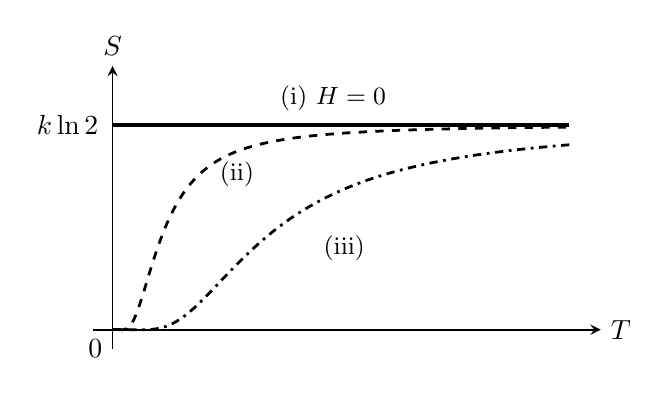
\begin{tikzpicture}[>=stealth, thick, scale=1.0]
  % Axes
  \draw[->, line width=0.65pt] (-0.25, 0) -- (6.2, 0) node[right] {$T$};
  \draw[->, line width=0.65pt] (0, -0.25) -- (0, 3.35) node[above] {$S$};
  \node[below left] at (0, 0) {$0$};

  % Horizontal asymptote k ln 2 at y = 2.6
  % (i) H = 0: S = k ln 2 (solid thick)
  \draw[line width=1.1pt] (0, 2.6) -- (5.8, 2.6);
  \node[left] at (-0.05, 2.6) {$k\ln 2$};
  \node[above, font=\small] at (2.8, 2.65) {(i) $H = 0$};

  % Overflow-free exact spin-1/2 entropy:
  % ln(2 cosh u) - u tanh u = ln(1 + exp(-2u)) + 2u * exp(-2u) / (1 + exp(-2u)), u = c / T
  % (ii) small finite H: c = 0.7
  \draw[line width=1.0pt, dashed, domain=0.08:5.8, samples=120, smooth]
    plot (\x, {2.6 * (ln(1 + exp(-1.4/\x)) + (1.4/\x)*exp(-1.4/\x)/(1 + exp(-1.4/\x))) / ln(2)});
  \draw[line width=1.0pt, dashed] (0, 0) -- (0.08, 0);
  \node[font=\small] at (1.58, 1.98) {(ii)};

  % (iii) large H: c = 2.2
  \draw[line width=1.0pt, dash dot, domain=0.20:5.8, samples=120, smooth]
    plot (\x, {2.6 * (ln(1 + exp(-4.4/\x)) + (4.4/\x)*exp(-4.4/\x)/(1 + exp(-4.4/\x))) / ln(2)});
  \draw[line width=1.0pt, dash dot] (0, 0) -- (0.20, 0);
  \node[font=\small, below right] at (2.55, 1.32) {(iii)};
\end{tikzpicture}
\end{document}
